
\documentclass{beamer}
\mode<presentation>
\usepackage{amsmath}
\usepackage{amssymb}
%\usepackage{advdate}
\usepackage{graphicx}
\graphicspath{{../figs/}}
\usepackage{adjustbox}
\usepackage{subcaption}
\usepackage{enumitem}
\usepackage{multicol}
\usepackage{mathtools}
\usepackage{listings}
\usepackage{url}
\def\UrlBreaks{\do\/\do-}
\usetheme{Boadilla}
\usecolortheme{lily}
\setbeamertemplate{footline}
{
  \leavevmode%
  \hbox{%
  \begin{beamercolorbox}[wd=\paperwidth,ht=2.25ex,dp=1ex,right]{author in head/foot}%
    \insertframenumber{} / \inserttotalframenumber\hspace*{2ex} 
  \end{beamercolorbox}}%
  \vskip0pt%
}
\setbeamertemplate{navigation symbols}{}
\let\solution\relax
\usepackage{gvv}
\lstset{
%language=C,
frame=single, 
breaklines=true,
columns=fullflexible
}

\numberwithin{equation}{section}
\title{9.8.3}
\author{AI25BTECH11001 - ABHISEK MOHAPATRA}
% \maketitle
% \newpage
% \bigskip
\begin{document}
{\let\newpage\relax\maketitle}
\renewcommand{\thefigure}{\theenumi}
\renewcommand{\thetable}{\theenumi}



	 	\textbf{Question}:
If a circle is passing through the point $\brak{a, b}$ and it is cutting the circle $x^2 + y^2 = k^2$ orthogonally, then the equation of the locus of its centre is
		
		\textbf{Solution:}

	Graph:
\begin{figure}[h!]
	\centering
	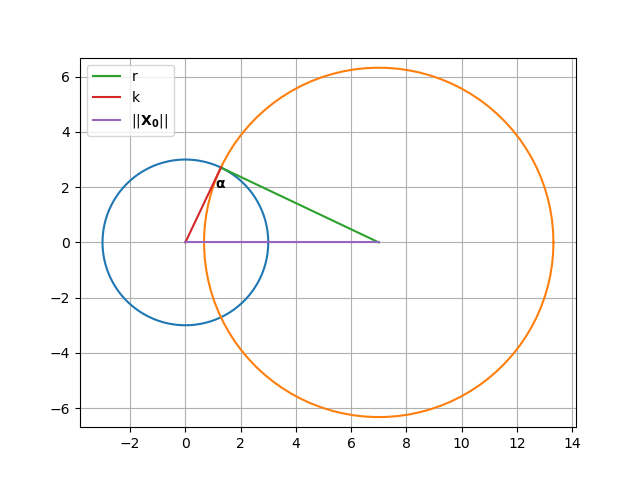
\includegraphics[width=0.55\linewidth]{img.png}
\end{figure}

Let center of the circle be $\vec{X_0}$ and radius of the circle be r.
So, equation of the circle be
\begin{align}
		\norm{\vec{X}-\vec{X_0}} = r
\end{align}
\begin{align}
		\norm{\vec{X}-\vec{X_0}}^2 = r^2
\end{align}
\begin{align}
		\brak{\vec{X}-\vec{X_0}}^\top\brak{\vec{X}-\vec{X_0}} = r^2
\end{align}
\begin{align}
		\norm{\vec{X}}^2-2\vec{X_0}^\top \vec{X}+\norm{\vec{X_0}}^2-r^2 = 0
\end{align}

And the other given circle be with center $\vec{0}$ and radius $k$.

As evident from the fig, for the circle to be orthogonal, $\angle\alpha$ = 90$^\circ$ and
\begin{align}
		r^2 + k^2 = \norm{\vec{X_0} - 0}^2= \norm{\vec{X_0}}^2
\end{align}
substituing in the equation,
\begin{align}
		\norm{\vec{X}}^2-2\vec{X_0}^\top \vec{X}+k^2 = 0
\end{align}
Putting th given point $\vec{\beta} = \myvec{a\\b}$
\begin{align}
		\norm{\vec{\beta}}^2-2\vec{X_0}^\top \vec{\beta}+k^2 = 0
\end{align}

So, option \textbf{$\brak{a}$} is correct.


Graph:
\begin{figure}[h!]
	\centering
	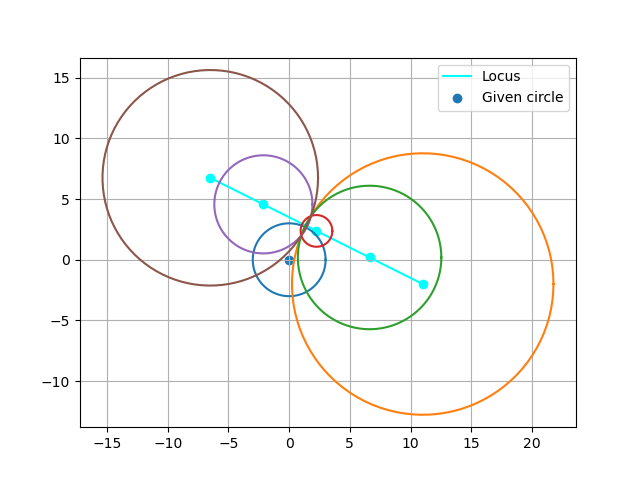
\includegraphics[width=0.7\linewidth]{img2.png}
\end{figure}

\end{document}




